
\documentclass[12pt, a4paper]{article}
\usepackage[margin=1in]{geometry}
\usepackage[utf8]{inputenc}
\usepackage[tablesfirst,nolists]{endfloat}
\usepackage{times}
\usepackage[flushleft]{threeparttable}
\usepackage{hyperref}
\usepackage{authblk}
\usepackage{setspace}
\usepackage{apacite}
\usepackage{caption}
\usepackage{graphicx}
\usepackage{titlesec}
\usepackage{color}
\usepackage{endnotes}
\usepackage{caption}
\usepackage{textcase}
\usepackage{booktabs}
\usepackage{titling}

\DeclareCaptionTextFormat{up}{\MakeTextUppercase{#1}}
\captionsetup{labelsep=newline,textformat=up}
\pagestyle{myheadings}
\title{}
\author{}
\date{}
\doublespacing
\renewcommand{\efloatheading}[1]{}

%    PRIMARY HEADING: Centered, capitalized, and italicized, with an extra return before and after.
%    SECONDARY HEADING: Flush left with title-style capitalization (first letter of each word) and italicized. You must have at least two sections beginning with a secondary heading; if there is only one, the heading should be excluded.
%    TERTIARY HEADING: Left justified and indented with sentence-style capitalization (first word only) in italics. Punctuate the heading with a period and begin the first line of the same section on the same line. If only one tertiary heading is used, the heading should be excluded.

\titleformat{name=\section,numberless}[hang]
  {\centering\itshape}
  {}
  {0em}
  {\Large\MakeUppercase}

\titleformat{name=\subsection,numberless}[hang]
  {\itshape}
  {}
  {0em}{}
  {\Large}

\titleformat{name=\subsubsection,numberless}[runin]
  {\itshape}
  {}
  {0em}{}
  {}

\let\footnote=\endnote

\providecommand{\keywords}[1]{\textbf{\textit{Keywords---}} #1}
%
\definecolor{orange}{rgb}{1,0.7,0.7}
\definecolor{green}{rgb}{0,1,0}
\newcommand{\NS}[1] {{\textcolor{green}{#1}}}
\newcommand{\AT}[1] {{\textcolor{cyan}{#1}}}
\newcommand{\TM}[1] {{\textcolor{orange}{#1}}}

\begin{document}
%The title should not exceed 25 words.
\title{A zero attraction effect in naturalistic choice}
%Zero attraction: A precisely zero attraction effect with naturalistic stimuli that meets Huber, Payne, and Puto's (2014) criteria

\author{Anna Trendl\\Department of Psychology, University of Warwick  \\  \href{mailto:a.trendl@warwick.ac.uk}{a.trendl@warwick.ac.uk}
\and Neil Stewart \\Warwick Business School, University of Warwick \\  \href{mailto:neil.stewart@wbs.ac.uk}{neil.stewart@wbs.ac.uk}
\and Timothy L. Mullett\\Warwick Business School, University of Warwick\\  \href{mailto:Tim.Mullett@wbs.ac.uk}{Tim.Mullett@wbs.ac.uk} }

\date{\today}


\begin{titlepage}
\maketitle
\thispagestyle{empty}

\clearpage
\thispagestyle{empty}
\begin{center}
\LARGE{A zero attraction effect in naturalistic choice}
\end{center}
%The abstract is limited to 175 words and summarizes the key components of the manuscript, offering the reader a sample of the manuscript.
\begin{abstract}
In the attraction effect, adding a dominated third option to a choice set of two options can reverse the preference for the original two options, and even increase one of the option's choice share. This constitutes a violation of the axioms of regularity and independence from irrelevant alternatives, which are core properties of any choice model in which the utility of each option is stable across choice sets. Consequently, in the past 20 years, the attraction effect has driven the development of a set of influential models of multiattribute choice. However, \citeA{Frederick2014} have recently claimed that the attraction effect is only limited to options with numerical attributes, and does not hold for choices between naturalistic options (e.g., snacks, movies) --- a claim which would severely undermine its theoretical importance. \citeA{Huber2014} criticised \citeauthor{Frederick2014}'s experiments, laying down a set of criteria that should be met by any experiment wishing to test for the attraction effect in real-world consumer choices. This article presents the first experiment that meets these criteria. The results show a precisely zero attraction effect.
%174 words now
\end{abstract}
%Keywords
\keywords{consumer choice, attraction effect, asymmetric dominance, attribute representation,  context effects}

%Include 4–5 primary keywords that best suit the topic of the manuscript; these do not necessarily need to match the “Topics/Methods” that are selected in Manuscript Central upon submission.

\end{titlepage}



%Main Text
%Please do not add any headers/footers on each page (other than the page number). Headings are text only (not numbered) and are formatted according to level.

%    PRIMARY HEADING: Centered, capitalized, and italicized, with an extra return before and after.
%    SECONDARY HEADING: Flush left with title-style capitalization (first letter of each word) and italicized. You must have at least two sections beginning with a secondary heading; if there is only one, the heading should be excluded.
%    TERTIARY HEADING: Left justified and indented with sentence-style capitalization (first word only) in italics. Punctuate the heading with a period and begin the first line of the same section on the same line. If only one tertiary heading is used, the heading should be excluded.
%Please make sure to use the correct heading style. When used, you must have more than one secondary heading per section (e.g., you may have a primary heading and two secondary/tertiary heading, but never a single secondary heading in a subsection).

%Do not label opening commentary as “Introduction.”

%Do not place tables and figures within the text. Rather, place them sequentially at the end of the text with titles above the tables and figures. Tables and figures must also be provided in their original format.

\newpage


\section*{The attraction effect}


Imagine that you are having a nice meal in a restaurant, and you are looking at the two dessert options available on the menu: cheesecake and pecan pie. You are torn between the creamy texture of the cheesecake, and the rich, nutty flavour of the pecan pie. You resolve to have the cheesecake. As the waiter approaches to take your order, he informs you that a third dessert option, apple pie---which you find quite bland---is also available today. But now you have changed your mind, and decide to order the pecan pie. \citeA{Tsetsos2010} give just this paradoxical example: the availability of the apple pie, which you do not want, makes you switch from cheesecake to pecan pie.

This is an example of the attraction effect (also known as asymmetric dominance effect). The presence of the apple pie (decoy) in the choice set makes you more likely to choose the pecan pie (target) over the cheesecake (competitor). In essence, it states that when the decision maker is indifferent between the target and the competitor (pecan pie and cheesecake in the example), the addition of an inferior decoy option that resembles the target (apple pie is similar to pecan pie, but is less liked by the decision maker) increases the likelihood that the target will be chosen.


The attraction effect is important, because it poses a challenge to all choice models that rely on the assumption that preferences can be represented on a cardinal utility scale. This assumption is called simple scalability, and is one of the consequences of Luce's choice axiom \cite{Luce1959}. Crucially, the attraction effect represents a violation of independence of irrelevant alternatives, which requires that the preference ranking of two options should not be affected by adding new options to the choice set. In addition, the attraction effect violates the axiom of regularity, which states that an option's choice probability cannot increase when the choice set is extended (\citeNP{Luce1977a}; \citeNP{Tversky1972a}). Therefore, the existence of the attraction effect implies that the utility of a choice option cannot be represented by a single internal magnitude that is invariant to the other options in the choice set.

Owing to its theoretical importance, the attraction effect has played a substantial role in the evolution of multialternative, multiattribute models of choice, with a significant number of various theoretical accounts being developed over the past 20 years (e.g., multialternative decision field theory, \citeNP{Roe2001a}; leaky competing accumulators, \citeNP{Usher2004b}; multialternative attentional drift-diffusion model,   \citeNP{Krajbich2010a}; range-normalization model, \citeNP{Soltani2012}; associative accumulation model, \citeNP{Bhatia2013b}; multiattribute linear ballistic accumulator, \citeNP{Trueblood2014a}; multialternative decision by sampling, \citeNP{Noguchi2018a}).

The first multiattribute choice experiments (e.g., \citeNP{Huber1982}; \citeNP{Simonson1992}) almost exclusively used stimuli presented as a set of numerical attributes (e.g., cars presented as numerical values for gas mileage and ride quality). However, recent experiments in multiattribute choice introduced what can perhaps be considered as more ecologically valid stimuli (e.g., movies presented as thumbnails and titles on Netflix, or photographs of popular snacks). Results from these experiments indicate that there might be significant differences in the processing of numerical and naturalistic stimuli. For example, \citeA{Bhatia2018b} find that, with naturalistic stimuli, the weighted additive model on a high-dimensional semantic representation generalises to new choices better than the simpler heuristic models, which perform so well on stimuli presented as sets of numerical attributes.

Recently, the existence of the attraction effect in choices that involve naturalistic options has become a contentious issue. Based on 38 experiments, \citeA{Frederick2014} presented a thorough investigation of the boundary conditions of the attraction effect. These experiments included choice options with numerical attributes, as well as complex, real-world stimuli (e.g., fruits, bottled water, apartments, etc.), and in some of these experiments, participants could even sample the choice options (e.g. squash, mints, popcorn). The overall conclusion of this study was that while the presence of the decoy seemed to affect choices when the options had numerical attributes, it was absent in experiments with more complex, naturalistic stimuli. In light of these results, \citeauthor{Frederick2014} posited that the psychological processes underlying decisions that involve options with numeric attributes are fundamentally different from those employed in decisions where the stimuli has a more naturalistic format. This conclusion was also supported by \citeA{Yang2014}, who reported difficulties replicating the attraction effect in experiments where the stimuli were pictorial, as opposed to cases where the attributes were presented numerically.

These two studies sparked considerable interest amongst decision making researchers, and led to the re-examination of the boundary conditions of the attraction effect. \citeA{Huber2014} discussed five critical conditions that can inhibit the attraction effect, and argued that many of these are present in the experiments reported by \citeA{Frederick2014} and \citeA{Yang2014}. The five critical conditions are to avoid: (1) strong prior preferences over the target and competitor, (2) inability to identify the dominance relationship  between the target and the decoy, (3) heterogeneity in prior preferences over the target and competitor, (4) an undesirable decoy and (5) a decoy that is too desirable. \citeA{Simonson2014a} further stressed the importance of the detection of the dominance relationship in observing the attraction effect, and also pointed out several other smaller, specific methodological shortcomings of the studies by \citeauthor{Frederick2014} and \citeauthor{Yang2014}.

Due to the theoretical significance of the attraction effect, it is important to know if the attraction effect is confined to choice settings with numerical stimuli presented in an attribute by alternative format. Arguably, while most consumer choices in the real world involve stimuli that are often presented in a rich naturalistic form \cite{Bhatia2018b}, development of formal models of choice have been almost exclusively reliant on results from experiments where the options have numerical attributes. In this article, we describe a test of the attraction effect with complex, naturalistic choice options, using an experimental methodology that addresses all of the critical conditions discussed by \citeA{Huber2014}. Using a movie choice task, we find no evidence for the attraction effect.

\section*{Testing the attraction effect with real-world stimuli}

The goal of this experiment was to test the attraction effect with naturalistic stimuli. We chose to use the most popular movies on IMDb as stimuli. Since movies are an integral part of Western culture, we can reasonably expect that most our participants will be sufficiently interested in the choice options. Furthermore, choosing between movies is a realistic, everyday task. In addition, the movie space is rich, and thus it allows us to create a wide range of unique choice triplets to test the attraction effect.

When the stimuli have numerical attributes, it is straightforward to construct choice triplets with a target, competitor and decoy. However, with naturalistic stimuli, this task is significantly more complicated. \citeA{Frederick2014} have also used movie stimuli in two of their experiments: they chose pairs of movies that are part of the same sequel or are starring the same actor (but have distinctly different genres) to create target-decoy pairs. With movie-sequel pairs, \citeauthor{Frederick2014} assumed that the sequel is the decoy, and the original is the target---which may, or may not have been true for their participants. With same-actor pairs, it is unclear how \citeauthor{Frederick2014} decided which movie should be the target.

Our novel experimental design takes individual preferences into account and ensures that decision makers are indifferent between the target and competitor and are able to clearly identify the inferiority of the decoy. To increase the statistical power of our experiment, we used a within-subjects design. We presented participants with both A, B, A' and B, A, B' triplet pairs (where X' is the dominated option). The triplet pairs were created from ``quadruplets'' (each made up of two choice triplets), using two distinctly different target-decoy pairs. Figure \ref{fig:quadruplets} shows an example of two choice triplets created from one such quadruplet.


\begin{figure}
\centering
\captionsetup{justification=centering}
		 \caption{Two choice triplets used in the experiment}
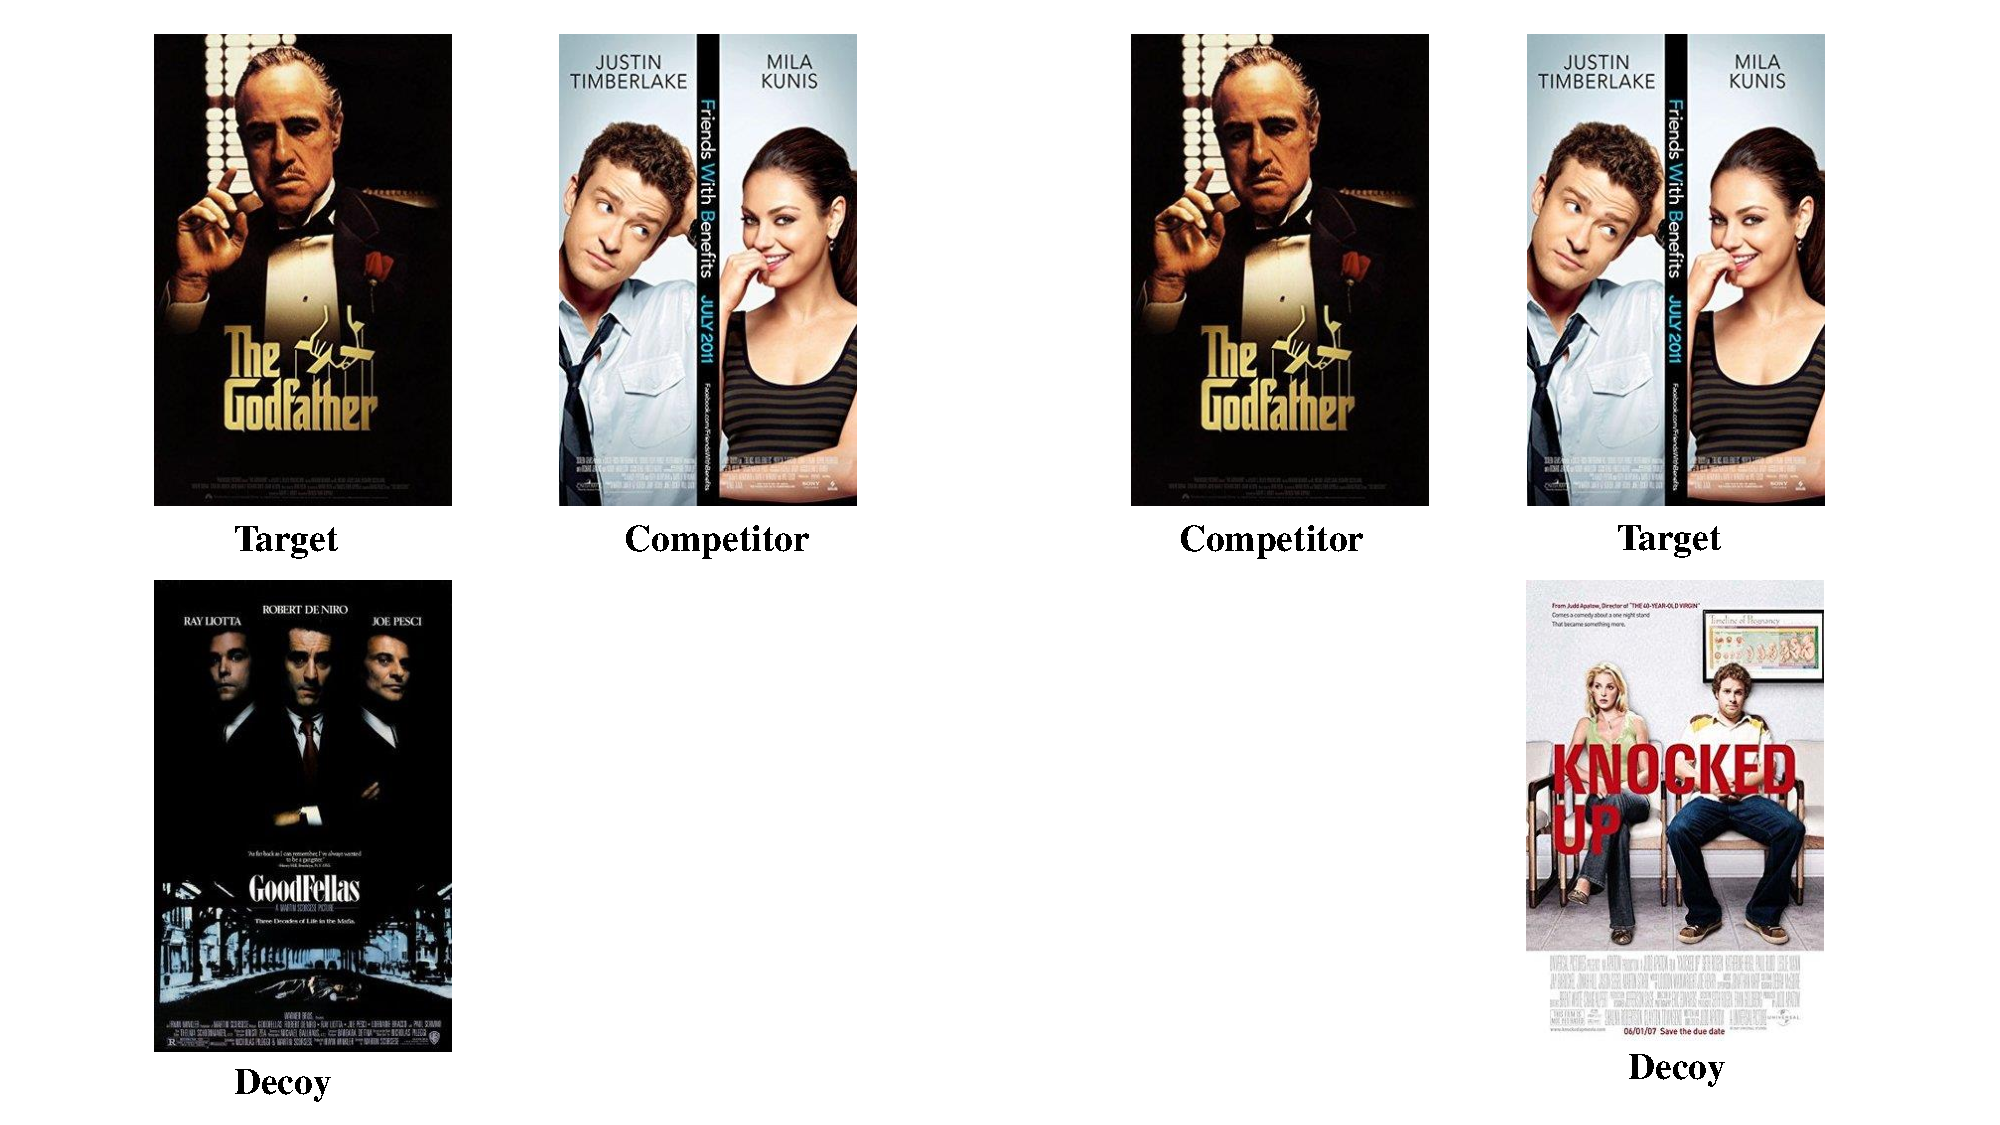
\includegraphics[width=1\textwidth]{figure1.pdf}
\label{fig:quadruplets}
\end{figure}

\subsection*{Method}

\subsubsection*{Preregistration.}
The study design, exclusion criteria and all the analyses were planned and registered before we collected any choice data. The pre-registration can be accessed \href{https://osf.io/fme6c/?view_only=31da4193689f4247a76af93b2f98fcef}{here}.

\subsubsection*{Candidate choice set selection.}

The list of movie triplets used in the experiment can be found \href{https://osf.io/fme6c/?view_only=31da4193689f4247a76af93b2f98fcef}{here}. The details of the construction of these triplets are somewhat arbitrary---a different recipe could have been used. However, the main point is that our triplets pass \citeauthor{Huber2014}'s \citeyear{Huber2014} criteria, as we detail below.

We first retrieved the most popular 40 movies from each of 10 distinct genre categories (romance, drama, sci-fi, thriller, comedy, horror, animation, fantasy, crime, action) from IMDb, so that we had 400 movies overall. The popularity of each movie was defined by the number of ratings it has received. We selected a wide range of genres to obtain a sufficiently rich stimuli space, as we wanted our participants to have a variety of preferences over our stimuli. We omitted any sequels.

Owing to the multidimensional nature of the stimuli, one of the main difficulties in creating attraction effect choice triplets from real-world objects is establishing a criterion for matching up similar objects. We used genre and sub-genre information from allmovie.com to create target-decoy pairs with many shared genres that are likely to be perceived as similar, and target-competitor pairs with no genre overlap that are likely to be perceived as different.

We conjectured that it will be harder to find movie pairs that will be perceived as similar, because any given movie is similar to a only a few movies, and dissimilar to all of the others. For this reason, we started the quadruplet creation with selecting potential target-decoy pairs.

The genre information on allmovie.com is very rich: compared to the 18 genre categories on IMDb, there are 156 genre and sub-genre categories, capturing many important aspects of the movies. Using this rich genre information, we created a movie by movie ($400 \times 400$) matrix, where each cell was the number of overlapping genre categories between the two movies. We selected a movie pair as target-decoy candidate if, for a given target candidate movie, the number of overlapping genres with a candidate decoy was equal to the maximum overlap seen for that target across all candidate decoy movies. This resulted in 2,271 target-decoy candidate movie pairs overall.
We also added 806 movie pairs obtained from the mutually closest 10\% of movies based on a latent semantic analysis\footnote{The latent semantic analysis assesses the similarity of two items based on the text associated with them. For this analysis, we used the summary text about the movies as well as plot keywords, actor and director names, all retrieved from IMDb.} that were not already in our list of target-decoy candidates. The rationale behind using semantic proximity as an additional criterion was to capture movie pairs that are very close to each other in terms of the story themes, but are not the closest on the genre dimension. Overall, we had 3,011 unique target-decoy candidate pairs at this point.

We then reduced the size of this list by selecting the most similar movie pairs. This was done manually by two researchers, who independently judged the similarity of each movie pair (not similar at all/similar). We then only kept the movie pairs that were judged as similar by both researchers, weeding out the movie pairs that were obviously not similar, resulting in 1,242 target-decoy candidates. We then divided the 1,242 pairs into six groups of 207 pairs, and ran a pilot study where we asked 60 participants to rate the similarity of a randomly chosen group of movie pairs, obtaining 10 independent similarity ratings for each of the 1,242 target-decoy candidates. Participants rated the similarity of each movie pair on a 1--7 scale, which also included a ``don't know'' option. Figure \ref{fig:exp2_pilot}  shows the distribution of the average similarity ratings for each movie pair.

\begin{figure}[htb!]
\centering
\captionsetup{justification=centering}
		\caption{The distribution of the average similarity rating for each target-decoy candidate pair (N = 1242). The dotted line is the cut-off value for accepting a movie pair as similar}
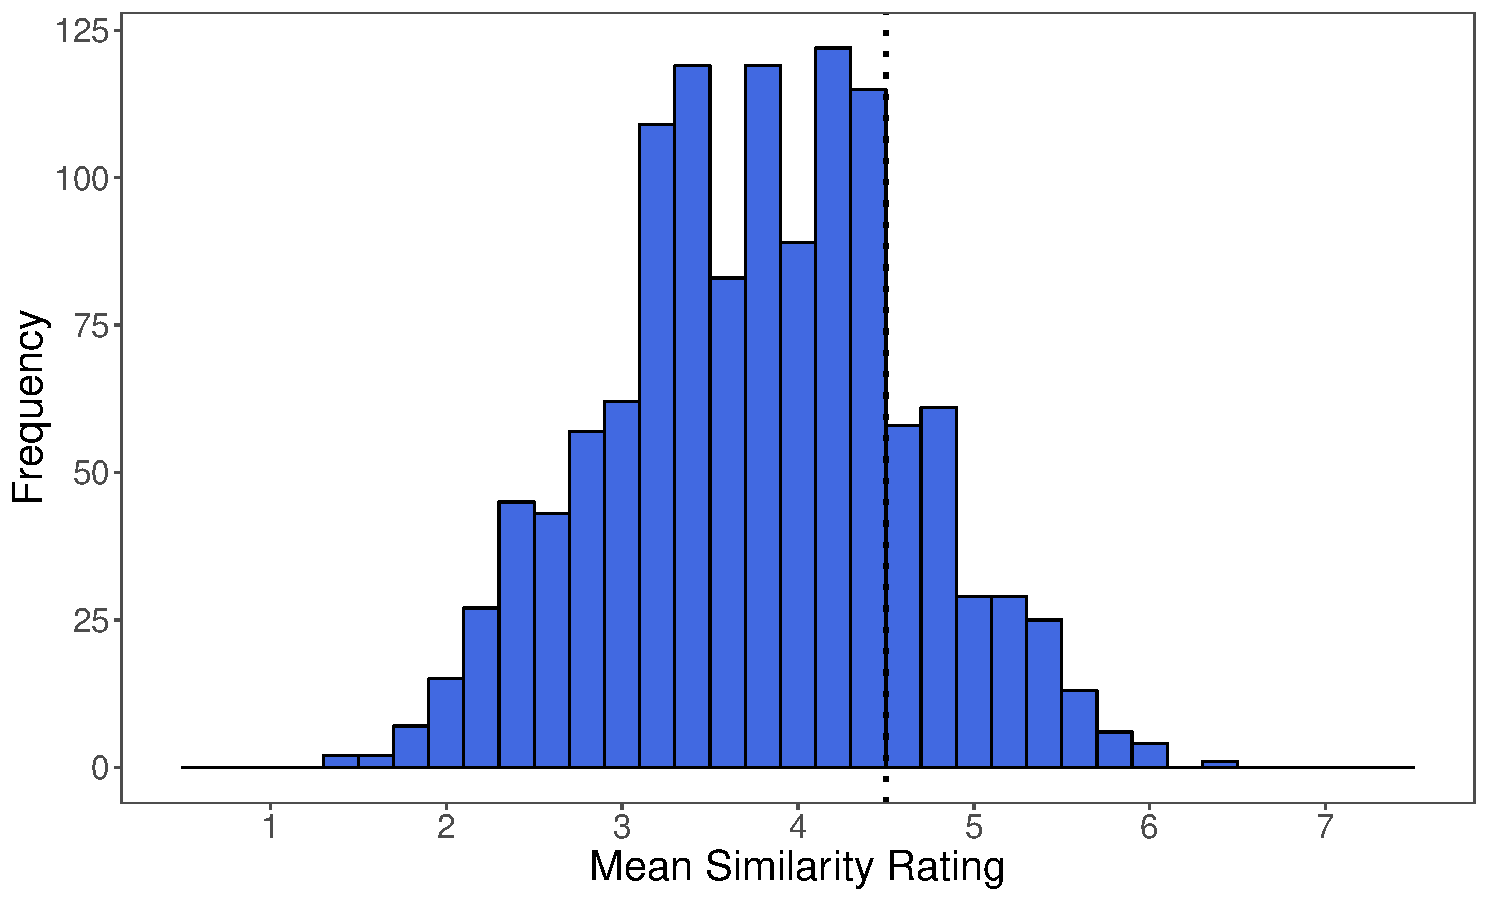
\includegraphics[width=0.9\textwidth]{figure2.pdf}
\label{fig:exp2_pilot}
\end{figure}

We decided to only use movie pairs with ratings that are equal to or higher than 4.5, which corresponds to the upper 20\% of the similarity rating distribution (253 movie pairs). This procedure intended to ensure that our target-decoy pairs will be perceived as similar by most people.

Having created the target-decoy pairs, the next step in creating the quadruplets was to create target-competitor pairs. Since each quadruplet consists of two target-decoy pairs, we decided to pair up the 253 target-decoy pairs to create the quadruplets. To do this, we first created a target-decoy pair by target-decoy pair matrix (253x253), where each cell was the number of overlapping genre categories (obtained from IMDb) between the two movie pairs. For example, considering the comparison between target-decoy pair 1 (consisting of Movie A and Movie B) and target-decoy pair 2 (consisting of Movie C and Movie D), we summed the number of genre overlaps between movies A-C, A-D, B-C and B-D. We then selected the unique target-decoy pairs that had no genre overlap with each other. This resulted in 20,022 quadruplets, each of which is a combination of four movies (created from two movie pairs, where each movie is similar to its pair, but is distinctly different from the two movies in the other pair), created from 231 unique movies. The quadruplets used for each participant are based upon their own ratings of the 231 movies, as we describe below.

\subsubsection*{Experimental procedure.}

The experiment consisted of three stages: rating stage, choice stage, and a similarity rating stage. In the rating stage, we asked for participants' subjective evaluations over the 231 movies (``How do you personally rate this movie?'') on a scale from 1 (worst) to 7 (best). We also asked whether the participant had seen the movie before. The 231 movies were presented in a random order for each participant. The rating stage took about 15--20 minutes.

Before the choice stage, we created a bespoke set of movie triplets for each participant using their ratings from the rating stage. First, based on each participant's preference ratings, we identified the subset of quadruplets where: (a) the target and competitor were both rated 4, both rated 5, both rated 6, or both rated 7, and (b) the two decoy movies were rated at least 3 points lower than the two target candidates. Note that we did not require the two decoys in the quadruplet to have the same rating, as it would have severely limited the number of eligible quadruplets (e.g., we allowed for quadruplets with ratings 7,7 for the two targets and 4,1 for the two decoys respectively), but we controlled for this difference in our analysis.

We then selected the subset of quadruplets where all of the movies had been seen or none of the movies had been seen, to make sure that choice behaviour will not be governed by differences in familiarity with the movies. The result was a bespoke subset of quadruplets for each participant, where the target/competitor movies had the same rating, and the decoy movies were rated worse. However, we did not want the same movie to appear twice as a target/competitor for one participant, and for this reason we used a sequential elimination technique: we first chose the quadruplet with the highest combined target-decoy similarity rating, then eliminated all quadruplets with the same target/competitor movies. We repeated these steps until we had a set a of quadruplets with unique target/competitor movies.

We only invited those participants back for whom we could create at least three unique quadruplets (corresponding to at least six attraction effect choice triplets, two per each quadruplet). In the choice stage, people were presented with the selected movie triplets in a random order, and were asked to choose the one they liked the most (see Figure \ref{fig:exp1_screenshot}).

\begin{figure}[htb!]
\centering
\captionsetup{justification=centering}
\caption{Choice stage}
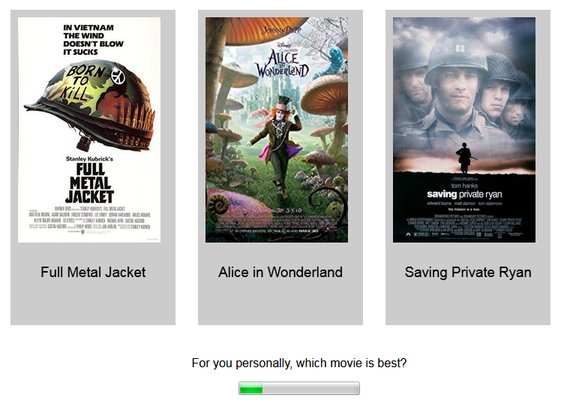
\includegraphics[width=0.8\textwidth]{rsz_exp1_choicestage.png}
\label{fig:exp1_screenshot}
\end{figure}

In the final, similarity stage, we asked participants to rate the similarity of all target-decoy and target-competitor pairs on a scale from 1 (least similar) to 7 (most similar), where a "don't know" option was also included. Information collected in this similarity rating stage was important to check that in the choice stage, participants perceived the target-decoy pairs as similar, and the target-competitor pairs as different.

We collected data in batches of 50, until we had choice data for at least a 100 participants (after all the exclusion criteria had been applied). At most, a few days have passed between the rating and choice stage. We recruited 297 participants from Prolific Academic who were paid £8 per hour. Out of the 297 participants who completed the rating stage, we could create quadruplets for 179 participants. Out of the 179 participants who were invited back, 152 took part in the choice stage of the experiment.

\subsubsection*{Exclusion criteria.} \label{exclusion_ref}

To conduct a rigorous test of the attraction effect, it is crucial that people take the task seriously and reveal their true preferences. Given that individually rating 231 movies can seem somewhat mundane, we specified a set of exclusion criteria to filter those people out who did not take the rating task sufficiently seriously. These were the following. We excluded people who fell into the fastest 5\% of the reaction time distribution, the lowest 5\% of the entropy distribution and the upper and lower 5\% of the autocorrelation distribution. Entropy refers to the diversity of the ratings, while autocorrelation takes into account the temporal pattern, and measures the extent to which a response depends on previous responses. Thus, this procedure filtered out response patterns where people (a) spent an unusually short time completing the task, or (b) did not use the whole of the ratings scale, or (c) often gave the same ratings for consecutive movies, or (d) were giving ratings randomly.

These exclusion criteria were validated in a pilot study, where we collected ratings for a set of books, and included repeat trials. The participants filtered out by these three criteria were the ones who gave the least consistent ratings to repeated stimuli (correlation r $<$ .8).

When we applied these exclusion criteria to our sample of 152 people, 17 participants were filtered out, leaving a sample of 2,148 choices from 135 participants.


\subsection*{Results}

The median number of choice trials per participant was 16 (range 6--54), and 84\% of participants were presented with at least 8 choice trials. The decoy was only chosen in 4.3\% of the trials. In addition, 72\% of participants never chose the decoy, and only 2\% chose it in more than 25\% of the trials. This indicates that participants were able to identify the dominated decoy in the choice stage.

In the attraction effect, the decoy increases the choice share of the target at the expense of the competitor. Figure \ref{fig:exp2_res} shows the proportions of trials where the target was chosen instead of the competitor (excluding all trials where the decoy was chosen, as specified in our preregistration). Each point corresponds to a participant. The mean proportion of trials where the target was chosen is M=.50, 95\% CI [.49--.51], which demonstrates that participants were almost perfectly indifferent between the target and the competitor, and that the attraction effect is virtually zero. A one-sample $t$-test shows that the proportion of trials where the target was chosen does not differ significantly from .5, $t(134)=.44$, $p=.67$.

\begin{figure}[htb!]
\centering
\captionsetup{justification=centering}
		\caption{The proportion of trials where the target was chosen instead of the competitor. Each dot is a participant. Dots are jittered slightly. The red dot and error bars show the bootstrapped mean and 95\% CI}
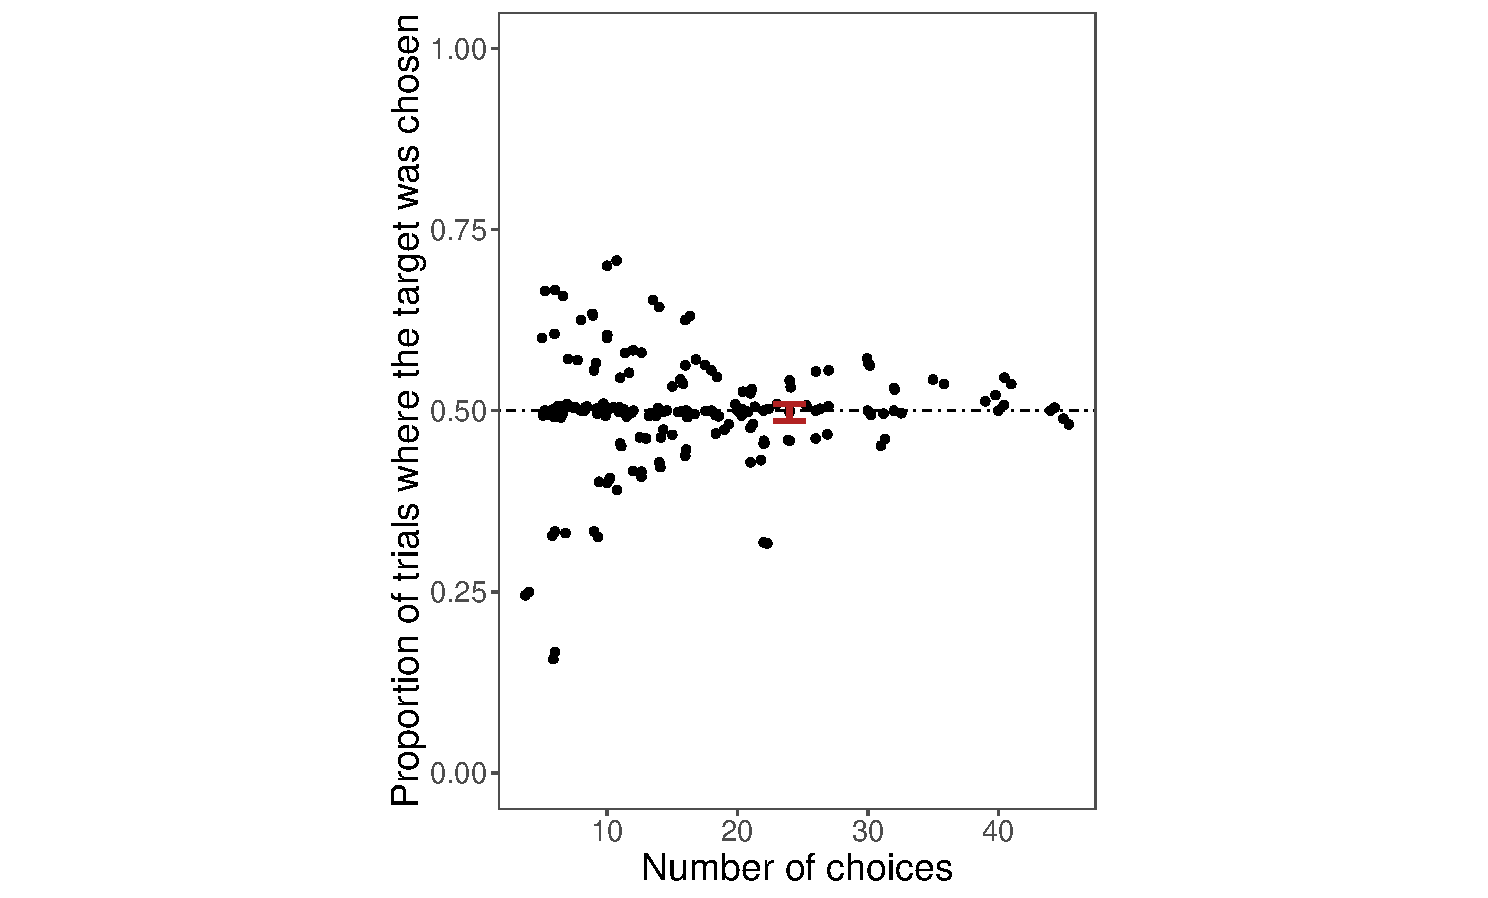
\includegraphics[width=0.9\textwidth]{figure4.pdf}
\label{fig:exp2_res}
\end{figure}

We created the choice triplets carefully to ensure that the target-decoy pairs were similar, and the target-competitor pairs were different. To check that our participants indeed perceived the triplets this way, we compared the distribution of the target-decoy and target-competitor similarity ratings. As Figure \ref{fig:exp2_similarityratings} shows, the overwhelming majority of target-competitor pairs were perceived as not similar, while the majority of target-decoy pairs were perceived as similar, as we intended.

\begin{figure}[htb!]
\centering
\captionsetup{justification=centering}
		\caption{Distribution of the target-competitor and target-decoy similarity ratings}
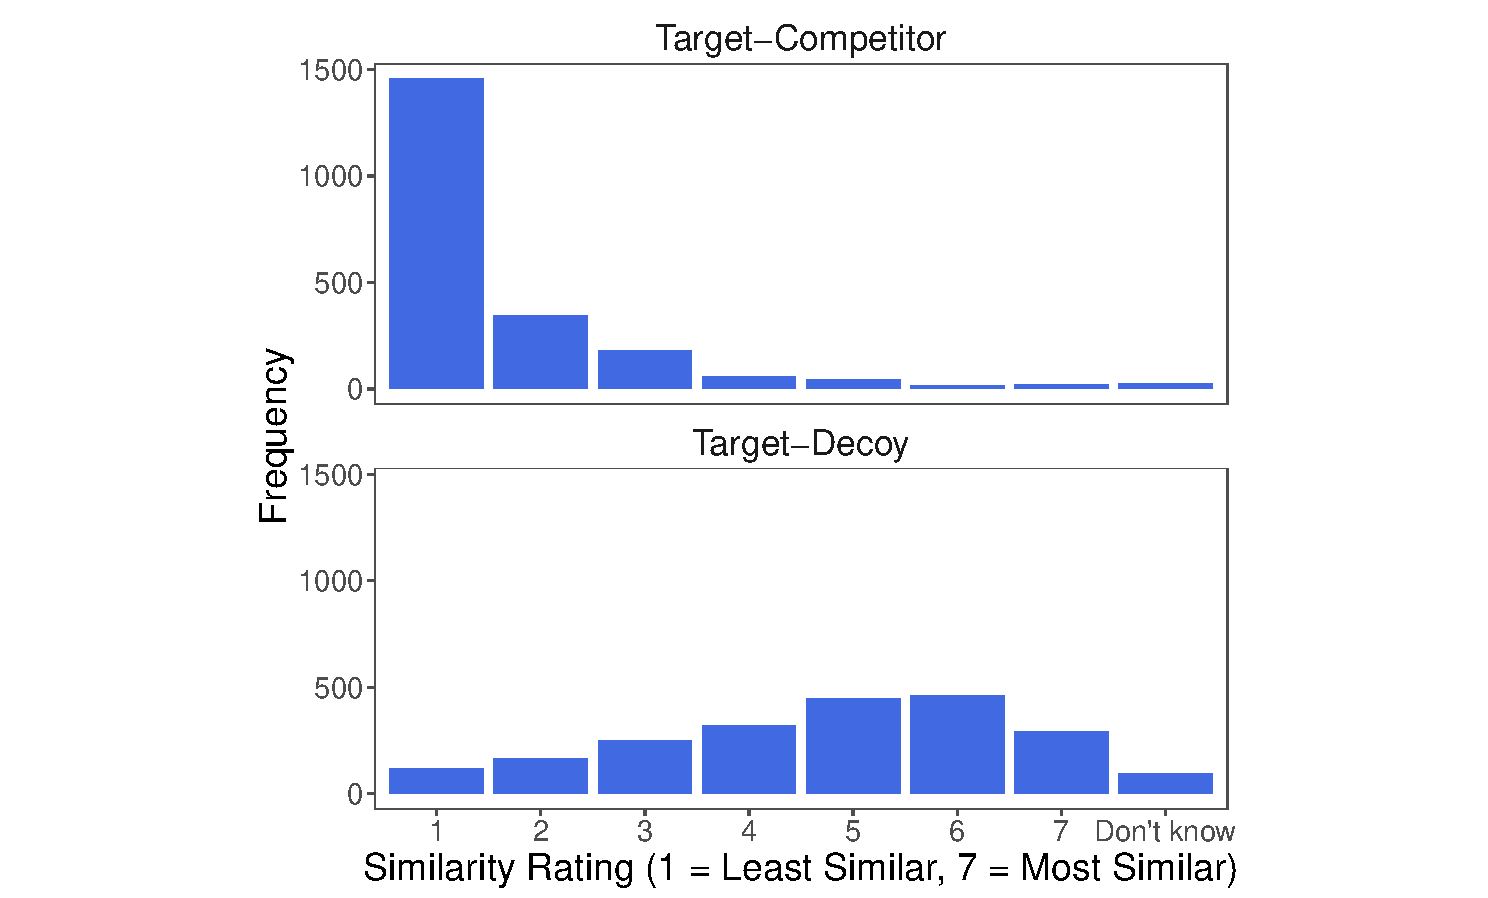
\includegraphics[width=0.8\textwidth]{Figure5.pdf}
\label{fig:exp2_similarityratings}
\end{figure}

We estimated the likelihood of choosing the target whilst accounting for subject-specific variability. Model 1 in Table \ref{latentattr_exp2reg} is an intercept-only mixed effects logistic regression with by-subjects intercepts. The odds of 1 for choosing the target over the competitor reflect equal preference for the target and competitor, and corresponds to the choice proportion of .5 in Figure \ref{fig:exp2_res}. Using Model 1, the overall probability of choosing the target is .50, 95\% CI [.48--.52], as we see in the mean over subject proportions from Figure \ref{fig:exp2_res}.

We also ran a mixed effects logistic regression with by-subjects intercepts to investigate how participants' target-decoy and target-competitor similarity ratings, familiarity with the movies, and target-decoy preference rating difference affect the likelihood of choosing the target (see Model 2 in Table \ref{latentattr_exp2reg}). The sample size is slightly smaller because people giving ``Don't Know'' ratings were not included. None of the ratings modulate the strength of the attraction effect. The overall probability of choosing the target is .50 95\% CI [.44--.55], with a slightly wider confidence interval. The conclusion from the two models and the simple mean over proportions is the same: we estimate a precisely zero attraction effect.

\begin{table*}[htb]
\centering
  \begin{threeparttable}
    \captionsetup{justification=centering}
    \caption{Odds ratios and 95\% CIs from two mixed-effects logistic models with subject-specific intercepts}
  \label{latentattr_exp2reg}
\begin{tabular}{@{\extracolsep{5pt}}lcc}
\\[-1.8ex]\hline
\hline \\[-1.8ex]
 & \multicolumn{2}{c}{\textit{Dependent variable:}} \\
\cline{2-3}
\\[-1.8ex] & \multicolumn{2}{c}{Target chosen} \\
 & Model 1 & Model 2 \\
\hline \\[-1.8ex]
 Intercept & 1.001 (0.918, 1.091) & 0.987 (0.802, 1.214) \\
  Seen all &  & 1.046 (0.690, 1.587) \\
  TC similarity rating &  & 0.960 (0.877, 1.050) \\
  TD similarity rating &  & 0.981 (0.895, 1.075) \\
  TD rating difference &  & 0.944 (0.863, 1.032) \\
 \hline \\[-1.8ex]
Observations & 2,055 & 1,953 \\
Log Likelihood & $-$1,424.417 & $-$1,352.312 \\
Akaike Inf. Crit. & 2,852.834 & 2,716.624 \\
Bayesian Inf. Crit. & 2,864.090 & 2,750.087 \\
\hline
\hline \\[-1.8ex]
%\textit{Note:}  & \multicolumn{2}{r}{$^{*}$p$<$0.1; $^{**}$p$<$0.05; $^{***}$p$<$0.01} \\
\end{tabular}
    \begin{tablenotes}
      \small
      \item Notes: $^{**}$p$<$0.05; ratings have been scaled; Seen all is coded 0.5 (Yes) and -0.5 (No); T - Target, C - Competitor, D - Decoy
    \end{tablenotes}
  \end{threeparttable}
\end{table*}

\section*{Discussion}

We tested for the attraction effect in a choice task with naturalistic choice options. We found that the presence of the decoy in the choice set did not alter preferences over the target and the competitor, as participants remained indifferent between the target and competitor. Our experiment is the first investigation to rigorously test the attraction effect with naturalistic stimuli whilst also addressing all of the criticisms raised in connection with \citeauthor{Frederick2014}'s experiments. 

First, our experimental design ensured participants' indifference between the target and the competitor, maximising the probability that choices will be constructed on the spot (rather than through relying on strong prior preferences), and that an attraction effect will occur. While one could argue that mnemonic processes arising from familiarity with the stimuli could have altered preferences in the choice stage, we did not detect any evidence for an attraction effect when participants were not familiar with the movies.

Second, we have strong evidence that the dominance relationship was perceived in our experiment. The target-decoy similarity ratings confirmed that our careful target-decoy selection process resulted in movie pairs that were perceived as similar. In addition, our choice set construction criteria ensured that the decoy was always rated at least 3 units lower than the target (and the competitor). Consequently, the decoy was only chosen in 4.3\% of the trials, which clearly shows that participants were able to spot and avoid the dominated option.

Third, by creating bespoke choice triplets based on the ratings, we avoided individual heterogeneity in preferences as a potential confound. In addition, we ensured that the decoy is not too desirable in comparison to the target. We also used a strict exclusion criteria to filter out participants who did not take the task sufficiently seriously, and with an average of 16 choice trials per participant, we avoided participant fatigue.

Finally, in our analysis, we controlled for familiarity with the choice options, perceived similarity of the target-decoy and target-competitor pair, and preference difference between the target and the decoy, but we found that none of these modulated or revealed an attraction effect.

To conclude, our results corroborate the findings of \citeauthor{Frederick2014} and \citeauthor{Yang2014}: we did not find evidence for the attraction effect with naturalistic stimuli.



\bibliographystyle{apacite}

\newpage

\bibliography{refs}

\newpage

\theendnotes

\newpage





\end{document}
